\chapter{La energía cinética y la seguridad vial}\label{ch:g9:kinetic-energy-safety}

Desde los juguetes de cuerda de tu infancia, la \omterm{def:g5:everyday-energy:energy}{energía} ha sido una
historia de reservas y de formas --- vívida, útil y sin números. La
espera termina ahora. La \omterm{def:g5:everyday-energy:energy}{energía} del movimiento recibe su fórmula,
la \omterm{def:g5:everyday-energy:energy}{energía} recibe su \omterm{def:g6:measurement-in-science:measuring}{unidad}, y la aritmética resulta
gobernar un asunto de vida o muerte: por qué un coche al doble de
\omterm{def:g7:motion-average-speed:formula}{velocidad} es cuatro veces más difícil de parar, y cuánto cuesta en
\omterm{def:g2:measuring-length:units}{metros} un solo segundo de despiste.

\section{La energía del movimiento}

\begin{definition}[El julio]\label{def:g9:kinetic-energy-safety:joule}
La \omterm{def:g5:everyday-energy:energy}{energía} --- en todas sus formas --- se mide en
\emph{julios}\index{julio} (\unit{J}), en honor del experimentador que
demostró que el propio \omterm{def:g5:heat-and-insulation:heat}{calor} es una forma de \omterm{def:g5:everyday-energy:energy}{energía}.
Anclas: levantar este libro del suelo al estante gasta unos pocos
julios; un corazón que late, alrededor de un julio por latido; una
tableta de chocolate almacena un millón de julios de \omterm{def:g5:everyday-energy:energy}{energía}
alimentaria.
\end{definition}

\begin{proposition}[Energía cinética]\label{prop:g9:kinetic-energy-safety:formula}
Un cuerpo de \omterm{def:g3:measuring-mass:mass}{masa} $m$ (en \unit{kg}) que se mueve a
\omterm{def:g7:motion-average-speed:formula}{velocidad} $v$ (en \unit{m/s}) lleva, en virtud de su movimiento, la
\emph{energía cinética}\index{energía cinética}
\[
E_k = \frac{1}{2} \times m \times v^2 ,
\]
en \omterm{def:g9:kinetic-energy-safety:joule}{julios}. Dos mandos, con potencias desiguales: doblar la
\omterm{def:g3:measuring-mass:mass}{masa} dobla $E_k$ --- pero doblar la \emph{\omterm{def:g7:motion-average-speed:formula}{velocidad}} la
\emph{cuadruplica}, porque la \omterm{def:g7:motion-average-speed:formula}{velocidad} entra al cuadrado. La
\omterm{def:g7:motion-average-speed:formula}{velocidad} es el mando peligroso.
\end{proposition}

\begin{example}[Primeros cálculos]\label{ex:g9:kinetic-energy-safety:first}
Un balón de \qty{0.45}{kg} a \qty{20}{m/s}: $E_k = 0.5 \times 0.45
\times 20^2 = \qty{90}{J}$. Un velocista de \qty{60}{kg} a
\qty{10}{m/s}: $0.5 \times 60 \times 100 = \qty{3000}{J}$. Un coche de
\qty{1000}{kg} a \qty{50}{km/h} --- convierte primero: $50 \div 3.6
\approx \qty{13.9}{m/s}$ --- $E_k = 0.5 \times 1000 \times 13.9^2
\approx \qty{9.7e4}{J}$: casi cien mil \omterm{def:g9:kinetic-energy-safety:joule}{julios}. El mismo coche a
\qty{100}{km/h}: cuatro veces más --- \qty{3.9e5}{J}. El aviso de la
fórmula, en números.
\end{example}

\begin{omfigure}
\begin{tikzpicture}
\begin{axis}[omaxis, width=10.2cm, height=6.0cm,
    xlabel={velocidad $v$ (\unit{km/h})},
    ylabel={$E_k$ (\unit{kJ})},
    xtick={0,30,50,70,90,110,130}, ytick={0,100,200,300,400,500},
    ymin=0, ymax=560, xmin=0, xmax=140, samples=100]
  \addplot[very thick, omThm, domain=0:135]
    {0.5*1000*(x/3.6)^2/1000};
  \addplot[only marks, mark=*, omDef] coordinates
    {(50,96.5) (100,385.8)};
  \node[right, font=\small, omDef] at (axis cs:38,130)
    {\qty{50}{km/h}};
  \node[left, font=\small, omDef] at (axis cs:99,400)
    {\qty{100}{km/h}: por cuatro};
\end{axis}
\end{tikzpicture}

{\small La \omterm{prop:g9:kinetic-energy-safety:formula}{energía cinética} de un coche de una tonelada frente a la
\omterm{def:g7:motion-average-speed:formula}{velocidad}: no una recta, sino una parábola --- el cuadrado de la
fórmula, dibujado. Doble \omterm{def:g7:motion-average-speed:formula}{velocidad}, cuádruple
\omterm{def:g5:everyday-energy:energy}{energía} de la que hay que deshacerse.}
\end{omfigure}

\begin{example}[Adónde la manda el frenado]\label{ex:g9:kinetic-energy-safety:brakes}
Para parar, un coche tiene que entregarle toda su $E_k$ a algo --- la
\omterm{def:g5:everyday-energy:energy}{energía} se pasa, no se borra nunca, como insistían las cadenas de
tu infancia. El agarre de los frenos la convierte en \omterm{def:g5:heat-and-insulation:heat}{calor}: los
discos se ponen ámbar tras las bajadas de montaña, y el olor a frenos
calientes \emph{es} \omterm{prop:g9:kinetic-energy-safety:formula}{energía cinética} jubilándose. En un choque, la
entrega es violenta e instantánea --- a chapa arrugada. Todos los
números de seguridad vial que vienen a continuación son esta
contabilidad: cuanto mayor la $E_k$, más larga, o más fea, su
jubilación.
\end{example}

\begin{omfigure}
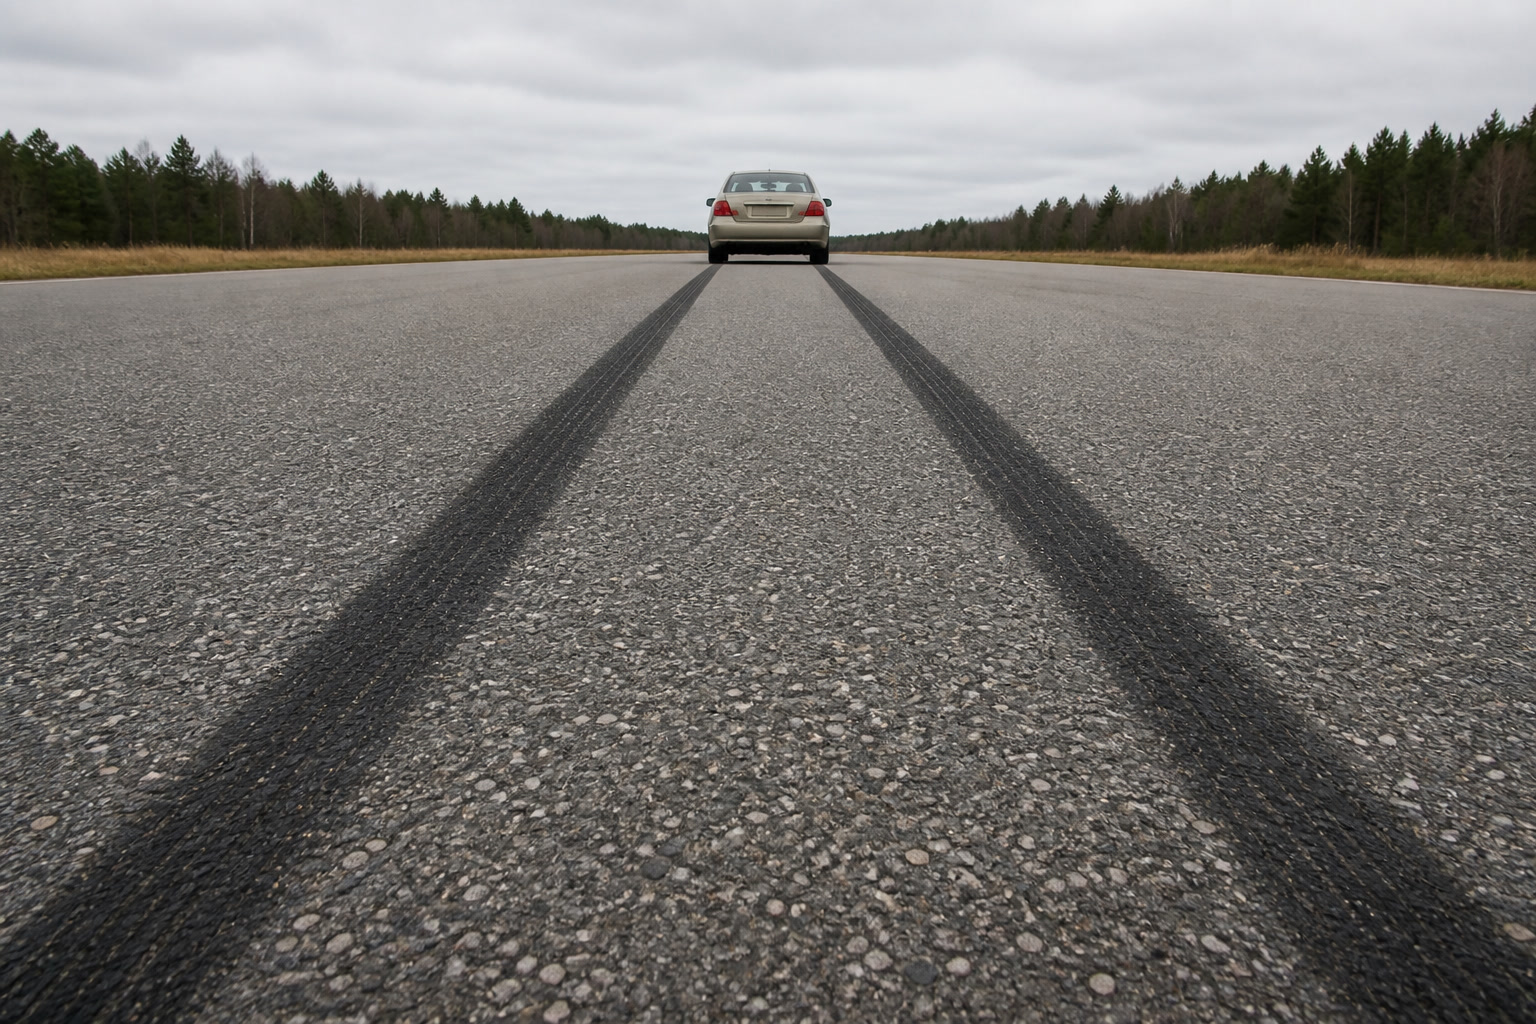
\includegraphics[width=0.55\linewidth]{images/book1/ai/g9-kinetic-skid-marks.jpg}

{\small Adónde fue la \omterm{prop:g9:kinetic-energy-safety:formula}{energía cinética}: los frenos y la carretera la convirtieron en \omterm{def:g5:heat-and-insulation:heat}{calor}, y los neumáticos firmaron el recibo.}
\end{omfigure}

\section{La distancia de parada}

\begin{proposition}[Parar = pensar + frenar]\label{prop:g9:kinetic-energy-safety:stopping}
Un \omterm{def:g4:conductors-insulators:conductor}{conductor} que ve un peligro no se para hasta después de dos tramos
de carretera:
\begin{enumerate}
  \item la \emph{distancia de reacción}\index{distancia de
        reacción}: la carretera recorrida mientras el cerebro se da
        cuenta y el pie se mueve --- alrededor de un segundo entero a
        la \omterm{def:g7:motion-average-speed:formula}{velocidad} de siempre, así que este tramo crece
        \emph{en proporción} a $v$;
  \item la \emph{distancia de frenado}\index{distancia de
        frenado}: la carretera que necesitan los frenos para jubilar
        la \omterm{prop:g9:kinetic-energy-safety:formula}{energía cinética} --- y, como $E_k$ lleva $v^2$, este
        tramo crece con el \emph{cuadrado} de la
        \omterm{def:g7:motion-average-speed:formula}{velocidad}: doble \omterm{def:g7:motion-average-speed:formula}{velocidad}, cuádruple
        carretera de frenado.
\end{enumerate}
Su suma, la \emph{distancia de parada}, es el número que se encuentra
con el niño que persigue la pelota.
\end{proposition}

\begin{example}[La tabla que debería tener todo conductor]\label{ex:g9:kinetic-energy-safety:table}
Carretera seca, \omterm{def:g4:conductors-insulators:conductor}{conductor} atento (un segundo de reacción; frenos
buenos):
\begin{center}
\begin{tabular}{l|c|c|c}
\omterm{def:g7:motion-average-speed:formula}{velocidad} & reacción & frenado & parada \\
\hline
\qty{50}{km/h} & \qty{14}{m} & \qty{13}{m} & \qty{27}{m} \\
\qty{90}{km/h} & \qty{25}{m} & \qty{40}{m} & \qty{65}{m} \\
\qty{130}{km/h} & \qty{36}{m} & \qty{85}{m} & \qty{121}{m}
\end{tabular}
\end{center}
Léela dos veces. A \omterm{def:g7:motion-average-speed:formula}{velocidad} de ciudad, un autobús y medio; a
\omterm{def:g7:motion-average-speed:formula}{velocidad} de autopista, una pista de atletismo entera y un quinto.
Y las proporciones confirman las dos leyes: la reacción crece como $v$
y el frenado como $v^2$ --- a \omterm{def:g7:motion-average-speed:formula}{velocidad} alta, el frenado devora el
total.
\end{example}

\begin{method}[Estimar una distancia de parada]\label{met:g9:kinetic-energy-safety:estimate}
\begin{enumerate}
  \item convierte la \omterm{def:g7:motion-average-speed:formula}{velocidad} a \unit{m/s} (divide los
        \unit{km/h} entre $3.6$);
  \item \omterm{prop:g9:kinetic-energy-safety:stopping}{distancia de reacción}: el viaje de un segundo --- el
        propio número en \unit{m/s}, en \omterm{def:g2:measuring-length:units}{metros};
  \item \omterm{prop:g9:kinetic-energy-safety:stopping}{distancia de frenado}: escala un ancla conocida con el
        cuadrado --- a partir de los \qty{13}{m} a \qty{50}{km/h},
        multiplica por $(v/50)^2$;
  \item suma, y compara con lo que ofrece de verdad la carretera de
        delante.
\end{enumerate}
Las carreteras mojadas doblan la parte del frenado; los \omterm{def:g4:conductors-insulators:conductor}{conductores}
cansados o distraídos estiran el segundo de reacción hacia los dos ---
rehaz la suma con los datos honrados.
\end{method}

\begin{example}[El precio de una miradita]\label{ex:g9:kinetic-energy-safety:glance}
Una miradita de dos segundos al móvil a \qty{90}{km/h}: el coche
recorre $2 \times 25 = \qty{50}{m}$ --- medio campo de fútbol ---
conducidos a ciegas, antes incluso de que empiece ningún segundo de
reacción. A \omterm{def:g7:motion-average-speed:formula}{velocidad} de ciudad, esa misma miradita gasta a ciegas
\qty{28}{m}: pasado el cruce, pasada la puerta del colegio. El
componente más peligroso del coche no lo mide ninguna fórmula de aquí:
la atención del \omterm{def:g4:conductors-insulators:conductor}{conductor}.
\end{example}

\begin{remark}[Cinturones, airbags y cascos]\label{rem:g9:kinetic-energy-safety:belts}
En una colisión, el coche se para en un \omterm{def:g2:measuring-length:units}{metro} de arrugarse ---
pero un pasajero sin cinturón continúa a toda \omterm{def:g7:motion-average-speed:formula}{velocidad} (la frase
tranquila del capítulo anterior, aplicada con crudeza) hasta que lo
para lo que le salga al paso: el salpicadero, el parabrisas, la
carretera. Los cinturones y los airbags paran el cuerpo a lo largo de
una distancia y un tiempo mayores, y jubilan su \omterm{prop:g9:kinetic-energy-safety:formula}{energía cinética}
con suavidad en lugar de toda de golpe; el casco del ciclista hace lo
mismo por el contenido insustituible del cráneo, con su espuma
aplastable comprando \omterm{def:g2:measuring-length:units}{centímetros} de parada suave. Ninguno de ellos
reduce tu $E_k$ ni un \omterm{def:g9:kinetic-energy-safety:joule}{julio} --- lo que hacen es civilizar su
jubilación.
\end{remark}

\section{Ejercicios}

\begin{exercise}[$\star$]\label{exo:g9:kinetic-energy-safety:1}
Da la \omterm{def:g6:measurement-in-science:measuring}{unidad} de \omterm{def:g5:everyday-energy:energy}{energía} y dos de sus anclas, y escribe la
fórmula de la \omterm{prop:g9:kinetic-energy-safety:formula}{energía cinética} con sus \omterm{def:g6:measurement-in-science:measuring}{unidades}.
\end{exercise}

\begin{exercise}[$\star$]\label{exo:g9:kinetic-energy-safety:2}
Calcula $E_k$: una liebre de \qty{2}{kg} a \qty{10}{m/s}; un jugador de
rugby de \qty{80}{kg} a \qty{5}{m/s}.
\end{exercise}

\begin{exercise}[$\star$]\label{exo:g9:kinetic-energy-safety:3}
¿Qué sube más la $E_k$ de un coche: añadirle media \omterm{def:g3:measuring-mass:mass}{masa} de carga
o subirle la \omterm{def:g7:motion-average-speed:formula}{velocidad} a la mitad más? Enseña los dos factores.
\end{exercise}

\begin{exercise}[$\star$]\label{exo:g9:kinetic-energy-safety:4}
Nombra los dos tramos de la distancia de parada y sus leyes de
crecimiento --- una proporcional y otra al cuadrado.
\end{exercise}

\begin{exercise}[$\star$]\label{exo:g9:kinetic-energy-safety:5}
A partir de la tabla del \omterm{def:g4:conductors-insulators:conductor}{conductor}: ¿qué fracción de la distancia de
parada es el frenado a \qty{50}{km/h} --- y a \qty{130}{km/h}? ¿Qué ha
cambiado?
\end{exercise}

\begin{exercise}[$\star$]\label{exo:g9:kinetic-energy-safety:6}
¿Adónde va la \omterm{prop:g9:kinetic-energy-safety:formula}{energía cinética} de un coche que frena? Cita el olor
y el resplandor --- y la ley de la infancia que le prohíbe
desvanecerse sin más.
\end{exercise}

\begin{exercise}[$\star$]\label{exo:g9:kinetic-energy-safety:7}
Calcula la \omterm{prop:g9:kinetic-energy-safety:stopping}{distancia de reacción} a \qty{36}{km/h},
\qty{72}{km/h} y \qty{108}{km/h} (con un segundo de \omterm{def:g4:conductors-insulators:conductor}{conductor} atento).
¿A qué pauta sencilla desfilan las respuestas?
\end{exercise}

\begin{exercise}[$\star$]\label{exo:g9:kinetic-energy-safety:8}
¿Por qué no reduce un cinturón de seguridad tu \omterm{prop:g9:kinetic-energy-safety:formula}{energía cinética}
--- y qué civiliza en su lugar?
\end{exercise}

\begin{exercise}[$\star\star$]\label{exo:g9:kinetic-energy-safety:9}
La \omterm{prop:g9:kinetic-energy-safety:stopping}{distancia de frenado} de una moto es de \qty{8}{m} a
\qty{30}{km/h}. Estímala a \qty{60}{km/h} y a \qty{90}{km/h} --- y di
la ley con la que has escalado.
\end{exercise}

\begin{exercise}[$\star\star$]\label{exo:g9:kinetic-energy-safety:10}
Los ayuntamientos bajan los límites de las zonas escolares de
\qty{50}{} a \qty{30}{km/h}. Compara las dos distancias de parada
(ancla: \qty{13}{m} de frenado a $50$; un segundo de reacción) --- y las
dos \omterm{prop:g9:kinetic-energy-safety:formula}{energías cinéticas}. ¿Qué comparación te parece más convincente para
un cartel?
\end{exercise}

\begin{exercise}[$\star\star$]\label{exo:g9:kinetic-energy-safety:11}
La lluvia dobla las \omterm{prop:g9:kinetic-energy-safety:stopping}{distancias de frenado}. Reconstruye la columna
de parada de la tabla del \omterm{def:g4:conductors-insulators:conductor}{conductor} para carretera mojada a $50$ y a
\qty{90}{km/h} --- ¿qué componente has doblado, cuál no, y por qué?
\end{exercise}

\begin{exercise}[$\star\star\star$]\label{exo:g9:kinetic-energy-safety:12}
Un camión de \qty{20000}{kg} rueda a \qty{90}{km/h}. Calcula su $E_k$
en notación científica; halla la \omterm{def:g7:motion-average-speed:formula}{velocidad} a la que un coche de
\qty{1000}{kg} igualaría esa \omterm{def:g5:everyday-energy:energy}{energía} (iguala las dos fórmulas ---
el álgebra es tuya este año); y concluye por qué existen rampas de
frenado de emergencia para camiones desbocados en las carreteras de
montaña mientras que no hay rampas así para los coches.
\end{exercise}

\section{Problema: la campaña de seguridad}

\begin{problem}[{Problema de fin de semana --- la clase diseña la
campaña de seguridad vial del pueblo; carteles comprobados con
fórmulas; las preguntas difíciles del
alcalde}]\label{pb:g9:kinetic-energy-safety:1}
El pueblo encarga una campaña con una condición: todos los números de
todos los carteles tienen que sobrevivir a una auditoría física. La
clase calcula. (Anclas: un segundo de reacción; \qty{13}{m} de frenado
a \qty{50}{km/h}, escalando con el cuadrado; \omterm{def:g3:measuring-mass:mass}{masa} del coche
\qty{1000}{kg}.)

\medskip\noindent\textbf{Parte I --- Cartel uno: ``50 y no 60''.}
\begin{enumerate}
  \item Calcula las dos \omterm{def:g7:motion-average-speed:formula}{velocidades} en \unit{m/s} (un decimal).
  \item ¿\omterm{prop:g9:kinetic-energy-safety:stopping}{Distancias de reacción} a las dos
        \omterm{def:g7:motion-average-speed:formula}{velocidades}?
  \item ¿\omterm{prop:g9:kinetic-energy-safety:stopping}{Distancias de frenado} a las dos (escala el ancla)?
  \item El titular del cartel: ``Diez \omterm{def:g6:measurement-in-science:measuring}{unidades} más de
        \omterm{def:g7:motion-average-speed:formula}{velocidad}: ¿cuántos \omterm{def:g2:measuring-length:units}{metros} más de parada?''. Rellena
        el número.
\end{enumerate}

\medskip\noindent\textbf{Parte II --- Cartel dos: ``El muro de la
\omterm{def:g7:motion-average-speed:formula}{velocidad}''.}
El diseño enseña las \omterm{def:g5:everyday-energy:energy}{energías} de choque como alturas de caída: un
choque a \omterm{def:g7:motion-average-speed:formula}{velocidad} $v$ ``es igual a'' caer desde la altura a la que
se ganaría esa misma \omterm{def:g5:everyday-energy:energy}{energía}.
\begin{enumerate}[resume]
  \item Calcula la $E_k$ del coche a \qty{50}{km/h} (de la Parte I)
        y a \qty{90}{km/h}.
  \item Los ilustradores necesitan alturas: caer desde \qty{1}{m}
        gana unos \qty{9.8}{kJ} para este coche ($m g h$ --- la otra
        fórmula del capítulo siguiente, tomada prestada antes de
        tiempo). ¿A qué alturas de caída corresponden las dos
        \omterm{def:g5:everyday-energy:energy}{energías} de choque? (Divide; redondea al \omterm{def:g2:measuring-length:units}{metro}.)
  \item ¿Qué edificios cotidianos igualan esas alturas? Redacta la
        línea del cartel.
  \item El alcalde objeta: ``Nadie se mete con el coche en un muro;
        los coches se arrugan y los cinturones sujetan''. Defiende
        la física del cartel concediéndole su parte de razón: ¿qué
        cambian las zonas de deformación y los cinturones, y qué
        número no cambian?
\end{enumerate}

\medskip\noindent\textbf{Parte III --- Cartel tres: ``Un segundo''.}
\begin{enumerate}[resume]
  \item A \qty{90}{km/h}, ¿cuántos \omterm{def:g2:measuring-length:units}{metros} cuesta un segundo de
        despiste antes de cualquier frenado? ¿Y una miradita de dos
        segundos al móvil?
  \item La variante del \omterm{def:g4:conductors-insulators:conductor}{conductor} cansado: la reacción estirada
        hasta dos segundos. Recalcula la distancia de parada
        completa a \qty{90}{km/h} y compárala con los \qty{65}{m}
        del \omterm{def:g4:conductors-insulators:conductor}{conductor} atento.
  \item Un concejal escéptico: ``Seguro que un segundo importa poco
        al lado de esos números tan grandes de frenado''. ¿A qué
        \omterm{def:g7:motion-average-speed:formula}{velocidades} se equivoca más --- a las bajas o a las
        altas? (Compara las leyes de crecimiento de los dos
        componentes.)
  \item Firma la campaña: tres líneas de pie de cartel, una por
        cartel, cada una con su fórmula en palabras llanas.
\end{enumerate}
\end{problem}
